\section{Implementation} \label{sec:implementation}
\subsection{Registers} \label{sec:implementation:registers}
This chapter will explain the implementation details of the register-module: the architecture of the driver module, data-pointer register, data, stack, loop-skip, instruction, instruction-pointer, and flag register. At the end of this chapter, we will provide the entire picture of the register-module.

\subsubsection{Overview}
In BFCPU, we omitted ALU because the only mathematical operation that brainf*ck can perform is adding and subtracting one. For the sake of simplicity, we decided to utilize 74LS193 and 74LS161 integrated chips to make individual registers. Both chips provide memory functionality along with incrementing of the value. Additionally, 74LS193 provides decrementing of the current value stored in the chip. It is important to note that F-R does not need any increment-decrement (INC-DEC) functionality. Thus, we used 74LS*** since it provides only the storage of a 4-bit value. 

\subsubsection{Common INC-DEC functionality problem}
Register module possesses a lot of INC and DEC pins that the control unit needs to manipulate in order to alter the value of registers. Driver module removes this inconvenience and serves as the common interface for all registers, and thus the entire register-module. The idea behind driver module is limiting all INC and DEC pins to one pair of DEC and INC pins, along with CLK (clock). If INC and DEC are both at low or high voltage, the mode of the selected register on the raising edge of the CLK is none, meaning that the value is neither incremented nor decremented. However, whenever INC-DEC pair has the digital value 01 or 10, the value of the selected register will be either incremented or decremented. The output of the driver module is the pair UP-DOWN that must be transmitted to an appropriate register\footnote{Or just UP signal for registers with 74LS161, as this chip can only increment}. Hence, we need a selecting interface to choose what register the computer is dealing with. The inner circuitry (see figure \ref{fig:registerModuleOverview}) accomplished this goal. A very general overview of the register-module is shown in the figure below. There are three select pins that provide us with 8 different possible paths, which is sufficient because we have less than 8 different registers.

\begin{figure}[H]
	\centering
	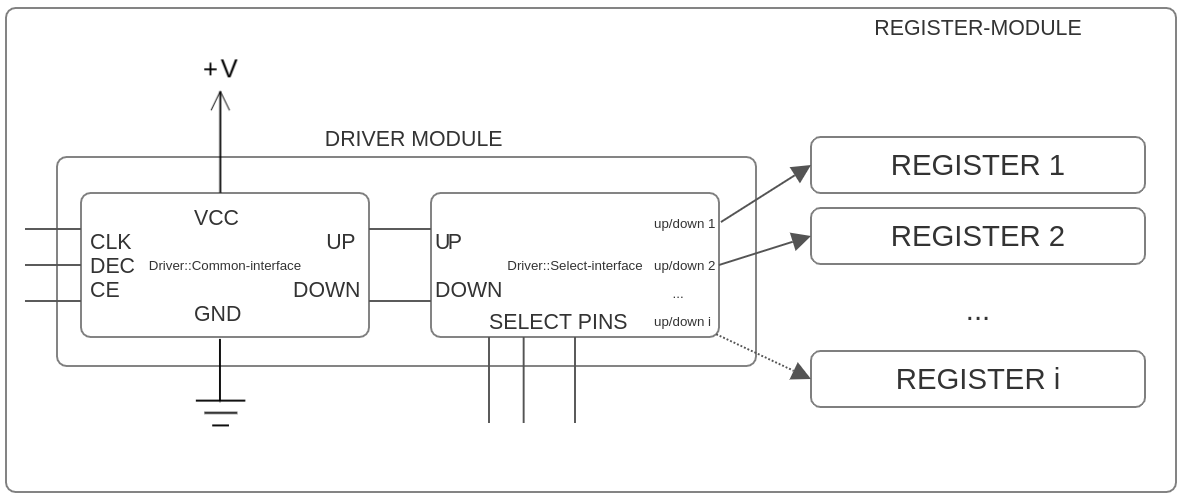
\includegraphics[width=0.9\textwidth]{img/register_module_overview}
	\caption{Register-module Overview}
	\label{fig:registerModuleOverview}
\end{figure}

\subsubsection{74LS193 Chaining}
Registers use 74LS193 (or 74LS161) to obtain storage and INC-DEC functionality. However, one 74LS193 chip has 4 bits whereas registers require 8 and 16 bits. Fortunately, 74LS193\footnote{Similar configuration works out for 74LS161, so we will not discuss it here} has a chaining ability: if CO (carry out) is connected to the UP pin of the other chip, and BO (borrow out) is connected to the DOWN pin, then we will obtain more bits available (see figure \ref{fig:registerModuleChaining}). This technique is used in every register that requires more than 4 bits.

\begin{figure}[H]
	\centering
	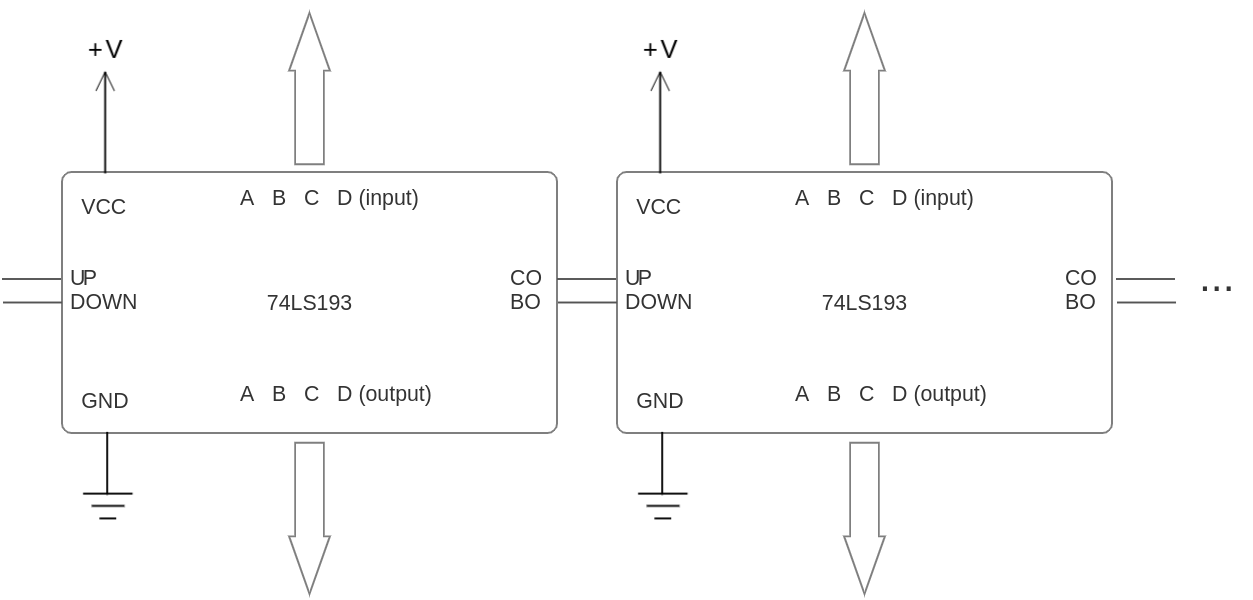
\includegraphics[width=0.9\textwidth]{img/register_module_chaining}
	\caption{Register-module 74LS193 chaining}
	\label{fig:registerModuleChaining}
\end{figure}

\subsubsection{Circuit: Driver Module}
When designing the computer, we had a lot of different ideas on the actual implementation of this module. Firstly, we utilized the demux-circuit, however, it was working only partially. Such problems as the potential propagation and incompatibility with 74LS193 were practically impossible to solve in a way that was sustainable and effective. Hence, we decided to remove this driver module design\footnote{See Appendix A(\ref{sec:appendix:old_driver_module_design})  to dive into the first driver module's circuitry}, and make another circuit, which is now the official part of the computer architecture. 

The idea behind this stable driver module is fairly simple: 
\begin{itemize}
	\item Set UP-DOWN\footnote{The output of the driver module} to HIGH whenever INC-DEC are both either high or low;
	\item Pulse UP and keep DOWN high, whenever INC is high and DEC is low;
	\item Pulse DOWN and keep UP high, whenever INC is low and DEC is high;
\end{itemize}
The actual implementation is visible in figure \ref{fig:actual_driver_module_implementation}, and the corresponding solutions are:
\begin{itemize}
	\item Common Interface:
	\begin{itemize}
		\item Use $$CLK + (INC \oplus DEC)$$ to eliminate any pulsing when INC-DEC have the same value;
		\item Connect the previous result with inverted INC-DEC into a NAND gate to achieve favorable behavior whenever INC-DEC have different values;
		\item Additional inverters are essential for the sake of compatibility with the registers and the select interface\footnote{The 3-to-8 demultiplexer that we used inverts the output};
	\end{itemize}
	\item Select Interface:
	\begin{itemize}
		\item Connect UP-DOWN pair to the 3-to-8 demultiplexer in order to route this pair to the selected register input;
	\end{itemize}
\end{itemize}

\begin{figure}[H]
	\centering
	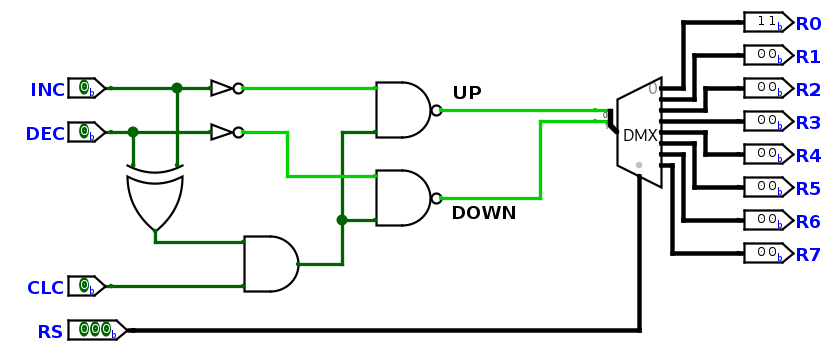
\includegraphics[width=0.9\textwidth]{img/actual_driver_module_implementation}
	\caption{The Actual Driver Module Implementation}
	\label{fig:actual_driver_module_implementation}
\end{figure}



\subsubsection{Circuit: Data Register}
Data register is a 8-bit valued flip-flop with both increment and decrement functionality. Therefore, we used 74LS193 chip. One essential property of the data register is that it also outputs a so-called zero flag (Z), which is 1 only if stored value is 0. The latter ability is implemented using OR gates and direct connection to stored bits. (see figure \ref{fig:dataRegisterImplementation})

\begin{figure}[H]
	\centering
	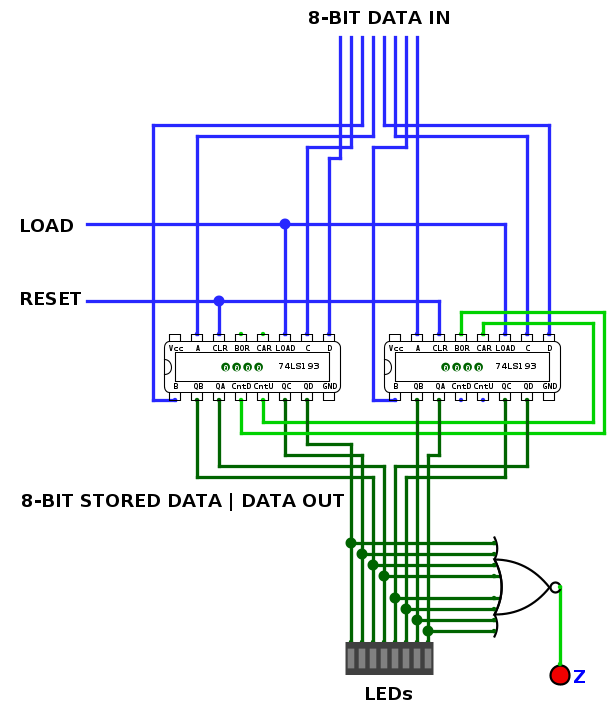
\includegraphics[width=0.9\textwidth]{img/data_register_implementation}
	\caption{Data, and Loop-Skip Register Implementation (\ref{sec:implementation:registers:loop_skip})}
	\label{fig:dataRegisterImplementation}
\end{figure}


\subsubsection{Circuit: Data-Pointer Register}
Data-Pointer register is a 8-bit valued flip-flop with both increment and decrement functionality. Therefore, we used 74LS193 chip. There is nothing very special about the data-pointer register, except that its output (value stored inside) is connected to the bus transceiver, but this applies for other registers as well\footnote{Implementation of the bus transceiver is fairly straightforward: as only outputs are connected along with DIR and CE (chip enable) pins as an input. Chips used is 74LS245}. (see figure \ref{fig:dataPointerRegisterImplementation})

\begin{figure}[H]
	\centering
	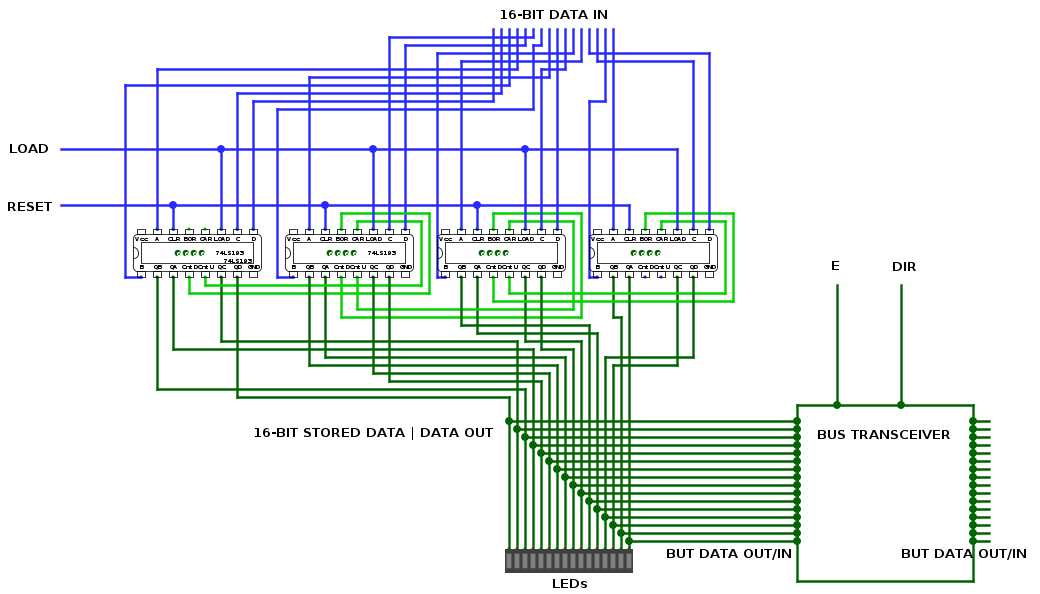
\includegraphics[width=0.9\textwidth]{img/data_pointer_register_implementation}
	\caption{Data-Pointer Register Implementation}
	\label{fig:dataPointerRegisterImplementation}
\end{figure}

\subsubsection{Circuit: Loop-Skip Register} \label{sec:implementation:registers:loop_skip}
Fundamentally, from the inner-circuit perspective loop-skip register (LS-R) has entirely the same implementation as the data-register (D-R): storage capacity of 8 bits, increment and decrement facilities, along with loop-flag\footnote{Loop-flag is the same as zero-flag for data-register, thus is implemented the same way as in the data register}. (refer to figure \ref{fig:dataRegisterImplementation})

\subsubsection{Circuit: Instruction Register}

\subsubsection{Circuit: Instruction-Pointer Register}

\subsubsection{Circuit: Stack Register}

\subsubsection{Circuit: Flag Register}



\subsection{Memory}
\subsection{Control Unit}
\subsection{Input}
\subsection{Output}

